\begin{frame}
 \frametitle{Sortes de synchronisation}
 
 \begin{tabular}{|cc|}
\hline
\textbf{Motifs biologiques} &

\\ \hline

\begin{tikzpicture}
\node[scale=0.7] (sai1) at (0,0){\begin{tikzpicture}[auto]
\path[use as bounding box] (-0.7,-0.3) rectangle (2.5,3);
\node[qgre] (a) at (0,2) {a};
\node[mod] (i) at (1,1) {i};
\node[qgre] (b) at (0,0) {b};
\node[qgre] (c) at (2,1) {c};
\node[es] (d) at (1,2.5) {activations indep.};

% arestorer
\path
 (a) edge[act] (i)
 (b) edge[act] (i)
 (i) edge[st]  (c);
\end{tikzpicture}};
\end{tikzpicture}


&

\begin{tikzpicture}
\node[scale=0.7] (sai1) at (0,0){\begin{tikzpicture}[auto]
\path[use as bounding box] (-0.7,-0.3) rectangle (2.5,3);
\node[qgre] (a) at (0,2) {a};
\node[mod] (i) at (1,1) {i};
\node[qgre] (b) at (0,0) {b};
\node[qgre] (c) at (2,1) {c};
\node[es] (d) at (1,2.5) {inhibitions indep.};

% arestorer
\path
 (a) edge[inh] (i)
 (b) edge[inh] (i)
 (i) edge[st]  (c);
\end{tikzpicture}};
\end{tikzpicture}

\\ \hline

\end{tabular}
\end{frame}

\begin{frame}
  \frametitle{Sortes de synchronisation}
  \framesubtitle{Raffinement structurel de la dynamique}
  %\framesubtitle{\tcite{PMR12-MSCS}}


\scalebox{\scaleex}{
\begin{tikzpicture}
\exphsyn
\end{tikzpicture}
}

\only<-14>{
\begin{liste}
  \item Comment introduire la \tval{Synchronisation} entre les sortes? \qex{$\PHfrappe{a_0 \wedge b_0}{c_2}{c_1}$}
\end{liste}
}

\end{frame}

\begin{frame}
\frametitle{Résultat avec la synchronisation}
% \begin{columns}
%  \begin{column}{0.3\textwidth}
% \scalebox{0.8}{
% \begin{tikzpicture}
% 
%  \node[scale=0.3] (syn) at (0,0) {
%  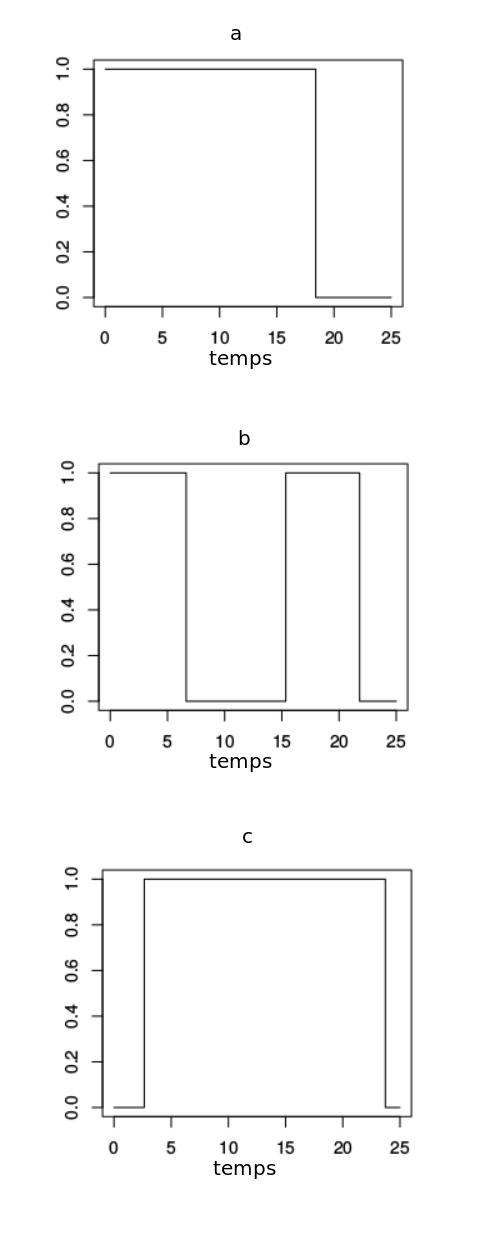
\includegraphics{figs/synchronisation.png}
%  oscillation.png: 400x1000 pixel, 72dpi, 14.11x35.27 cm, bb=0 0 400 1000
% };
% \end{tikzpicture}
% }
% 
% \end{column}
% 
% \end{columns}

\begin{figure}[!h]
   \begin{minipage}[c]{.46\linewidth}
      \centering
      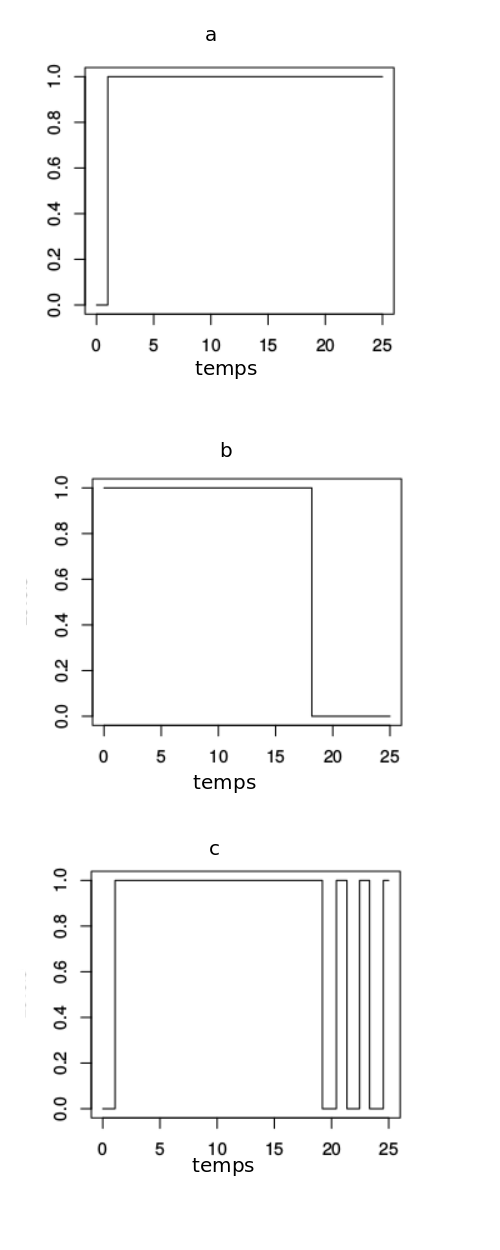
\includegraphics[scale=0.2]{figs/oscillation.png}
   \end{minipage} \hfill
   \begin{minipage}[c]{.46\linewidth}
   \centering
      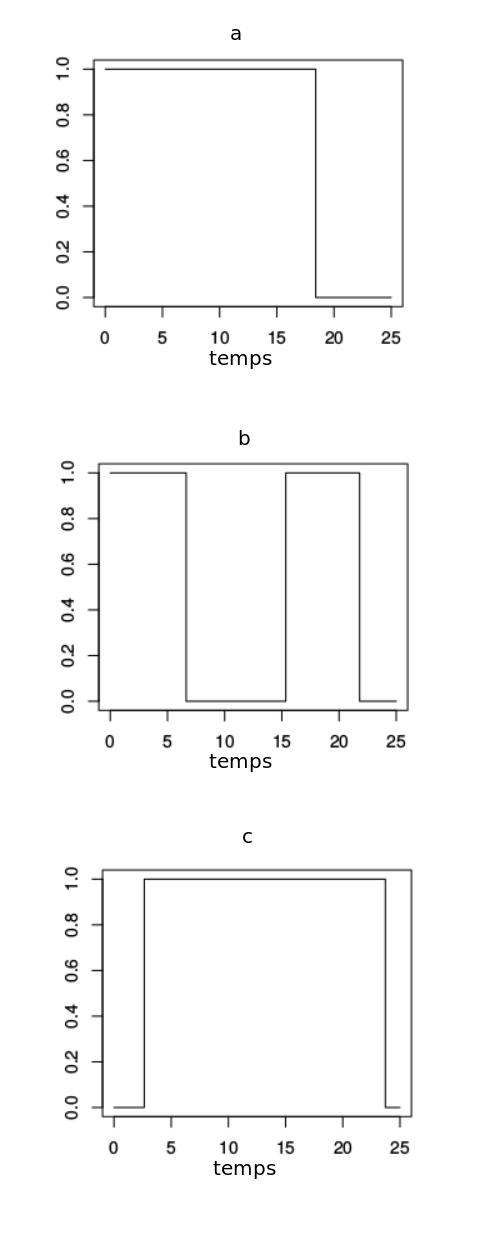
\includegraphics[scale=0.2]{figs/synchronisation.png}
   \end{minipage}
\end{figure}

\end{frame}

